\documentclass[10pt]{beamer}

\usepackage[utf8]{inputenc}
\usepackage[english]{babel}
\usepackage{amsfonts,amsmath,amssymb,bbold,dsfont}
\usepackage{calrsfs}
\usepackage[lined,boxed, ruled,vlined, french]{algorithm2e}
\usepackage{multirow}
\usepackage{mathtools,mathptmx}
\usepackage{empheq}
\usepackage{enumerate}
\usepackage{makecell}
\usepackage{tabularx}
\newcommand{\comment}[1]{}
\usepackage{hyperref}

% \usepackage[margin=1in,bindingoffset=15.5mm,heightrounded]{geometry}
% \usepackage{indentfirst}
\usepackage{geometry}

%% for images print/graphiques :
\usepackage{svg}
\usepackage{tikz}
\usetikzlibrary{tikzmark,calc,arrows,shapes,decorations.pathreplacing}
\tikzset{every picture/.style={remember picture}}
\usepackage{accents}
\usepackage{graphicx}
\usepackage{subcaption}

\newcommand\myubar[1]{\underaccent{\bar}{#1}}

%% text color 
\definecolor{ao(english)}{rgb}{0.0, 0.5, 0.0}

%% bibliographie :
% \usepackage{natbib}
% \usepackage[style=authoryear]{biblatex}
% \AtBeginBibliography{\scriptsize}


%% mes shortcuts
\newcommand{\aaa}{\alpha}
\newcommand{\bb}{\beta}


% \usepackage{iflang}
% \usepackage{enumitem}
% \setlist[itemize, 1]{label = \IfLanguageName{french}{\textendash}{\textbullet}}

\usepackage{geometry}

%%%%%%%%%%%%%%%%%%%%
%% theme of diapo %%
%%%%%%%%%%%%%%%%%%%% 
\usetheme{PaloAlto}
\usecolortheme{seahorse}
\addtobeamertemplate{footline}
{%
  \usebeamercolor[fg]{author in sidebar}
  \vskip-1cm\hskip10pt
  %\insertpagenumber\,/\,\insertpresentationendpage\kern1em\vskip2pt%
  \insertframenumber\,/\,\inserttotalframenumber\kern1em\vskip2pt%
}



\setbeamertemplate{blocks}[rounded][shadow=true]
%%%%title page
\defbeamertemplate*{title page}{customized}[1][]
{
    \begin{center}
    
    \usebeamerfont{title}
    {\LARGE \inserttitle\par}
    
   
    \vfill
     \begin{center}
        
\includegraphics[width = 0.5\linewidth ]{illustrations/logo_stackoverflow.png}
        \hspace{0.5cm}
    \end{center}   
    
    \vfill
    { \Large \insertauthor\par}
    \vfill
    {\large \insertdate\par}
   \end{center}
  }
  
%%%%% frame section
\AtBeginSection[]
{
\begin{frame}<beamer>
\frametitle{}
% \tableofcontents[
% %   currentsection,currentsubsection
%   currentsubsection,hideothersubsections,
% %   sectionstyle=show/show/shaded,
% %   subsectionstyle=show/show/hide]
%   sectionstyle=show/shaded,
%   subsectionstyle=show/show/
% ]
\tableofcontents[currentsection,currentsubsection, 
    hideothersubsections, 
    sectionstyle=show/shaded,
]
\end{frame}
}

\newif\iflattersubsect

\AtBeginSection[] {
    \begin{frame}<beamer>
    \frametitle{} %
    \tableofcontents[currentsection]  
    \end{frame}
    \lattersubsectfalse
}

\AtBeginSubsection[] {
    \iflattersubsect
    \begin{frame}<beamer>
    \frametitle{} %
    \tableofcontents[currentsubsection]  
    \end{frame}
    \fi
    \lattersubsecttrue
}


\beamertemplatenavigationsymbolsempty

%%%%% footer
\defbeamertemplate*{footline}{my footline}{
% 	\leavevmode%
	\hbox{%
		\begin{beamercolorbox}[wd=.3\paperwidth,ht=2.25ex,dp=1ex,center]{author in head/foot}%
			\usebeamerfont{author in head/foot}\insertshortauthor
		\end{beamercolorbox}%
		\begin{beamercolorbox}[wd=.6\paperwidth,ht=2.25ex,dp=1ex,center]{title in head/foot}%
			\usebeamerfont{title in head/foot}\insertshorttitle
		\end{beamercolorbox}%
		\begin{beamercolorbox}[wd=.1\paperwidth,ht=2.25ex,dp=1ex,center]{date in head/foot}%
			\insertframenumber{} / \inserttotalframenumber\hspace*{1ex}
	\end{beamercolorbox}}%
	\vskip 0pt%
    }
%\beamertemplatenavigationsymbolsempty
% \addto\captionsenglish{
%   \renewcommand{\labelitemi}{$\textendash$$}
% }
%%%%%%%%%%%%%%%%%%%%%%%%%%%%%%%%%%%%%%%%%%%%%%%%%%%%%%%%%%%%%%%%%%%%%%%%%%%%

\title{Projet 5 : }
\author{Claire Gayral}
%\institute{Université Claude Bernard, Lyon 1}
\date{Décembre 2021}

%%%%%%%%%%%%%%%%%%%%%%%%%%%%%%%%%%%%%%%%%%%%%%%%%%%%%%%%%%%%%%%%%%%%%%%
\begin{document}
\begin{frame}{}
    \frametitle{}
    \titlepage
\end{frame}
%%%%%%%%%%%%%%%%%%%%%%%%%%%%%%%%%%%%%%%%%%%%%%%%%%%%%%%%%%%%%%%%%%%%%%
\begin{frame}{Introduction}

\end{frame}
%%%%%%%%%%%%%%%%%%%%%%%%%%%%%%%%%%%%%%%%%%%%%%%%%%%%%%%%%%%%%%%%%%%%%%
\begin{frame}{Introduction - Plan}
    \tableofcontents
\end{frame}

%%%%%%%%%%%%%%%%%%%%%%%%%%%%%%%%%%%%%%%%%%%%%%%%%%%%%%%%%%%%%%%%%%%%%%
%%%%%%%%%%%%%%%%%%%%%%%%%%%%%%%%%%%%%%%%%%%%%%%%%%%%%%%%%%%%%%%%%%%%%%
\section{La mission}
%%%%%%%%%%%%%%%%%%%%%%%%%%%%%%%%%%%%%%%%%%%%%%%%%%%%%%%%%%%%%%%%%%%%%%
%%%%%%%%%%%%%%%%%%%%%%%%%%%%%%%%%%%%%%%%%%%%%%%%%%%%%%%%%%%%%%%%%%%%%%

\begin{frame}{Les données}
Les données d'entrée : 
\begin{itemize}
    \item 8 tables anonymisées avec des jointure possibles
    \item 2017-2018 
    \item En portugais\\
\end{itemize}
\vspace{0.5cm}
Les données de sortie :
\begin{itemize}
    \item Segmentation des clients
    \item Interprétation des types d'utilisateurs
    \item Solution actionnable par l'équipe marketing
    \item Proposition contrat de maintenance
\end{itemize}
\end{frame}
%%%%%%%%%%%%%%%%%%%%%%%%%%%%%%%%%%%%%%%%%%%%%%%%%%%%%%%%%%%%%%%%%%%%%%
\begin{frame}{Les données}
       \begin{center}
           \includegraphics[width=0.9\linewidth]{illustrations/kaggle_graph_link_datasets.png}
       \end{center}
\end{frame}
%%%%%%%%%%%%%%%%%%%%%%%%%%%%%%%%%%%%%%%%%%%%%%%%%%%%%%%%%%%%%%%%%%%%%%
%%%%%%%%%%%%%%%%%%%%%%%%%%%%%%%%%%%%%%%%%%%%%%%%%%%%%%%%%%%%%%%%%%%%%%
%%%%%%%%%%%%%%%%%%%%%%%%%%%%%%%%%%%%%%%%%%%%%%%%%%%%%%%%%%%%%%%%%%%%%%
\section{Analyse exploratoire}
%%%%%%%%%%%%%%%%%%%%%%%%%%%%%%%%%%%%%%%%%%%%%%%%%%%%%%%%%%%%%%%%%%%%%%
%%%%%%%%%%%%%%%%%%%%%%%%%%%%%%%%%%%%%%%%%%%%%%%%%%%%%%%%%%%%%%%%%%%%%%
%%%%%%%%%%%%%%%%%%%%%%%%%%%%%%%%%%%%%%%%%%%%%%%%%%%%%%%%%%%%%%%%%%%%
\begin{frame}{Exploration des tables}
       \begin{center}
           \includegraphics[width=0.9\linewidth]{illustrations/graph_all.png}
       \end{center}
\end{frame}
%%%%%%%%%%%%%%%%%%%%%%%%%%%%%%%%%%%%%%%%%%%%%%%%%%%%%%%%%%%%%%%%%%%%%%
%%%%%%%%%%%%%%%%%%%%%%%%%%%%%%%%%%%%%%%%%%%%%%%%%%%%%%%%%%%%%%%%%%%%%%
\subsection{Echelle Produit}
%%%%%%%%%%%%%%%%%%%%%%%%%%%%%%%%%%%%%%%%%%%%%%%%%%%%%%%%%%%%%%%%%%%%%%
%%%%%%%%%%%%%%%%%%%%%%%%%%%%%%%%%%%%%%%%%%%%%%%%%%%%%%%%%%%%%%%%%%%%%%
\begin{frame}{Exploration des tables - Produits }
\begin{minipage}{0.3\linewidth}
        \begin{center}
           \includegraphics[width=0.8\linewidth]{illustrations/graph_only_products.png}
        \end{center}
\end{minipage}
\begin{minipage}{0.68\linewidth}
\begin{itemize}
    \item Table \textit{products} :
    \begin{itemize}
        \item[$\textendash$] Description de produit
        \item[$\textendash$] Dimension de produit
        \item[$\textendash$] Catégorie de produit
    \end{itemize}
    \item Table \textit{order items} : 
    \begin{itemize}
        \item[$\textendash$] Nombre de produit commandé
        \item[$\textendash$] Prix des produits
        \item[$\textendash$] Fréquence d'achat
    \end{itemize}
\end{itemize}
\end{minipage}
\end{frame}
% %%%%%%%%%%%%%%%%%%%%%%%%%%%%%%%%%%%%%%%%%%%%%%%%%%%%%%%%%%%%%%%%%%%%%%
% \begin{frame}{Produits - valeurs manquantes }
% \begin{center}
%   \includegraphics[width=0.8\linewidth]{figures/analyse_exploratoire/set_n_KNN_impute_products.jpg}
% \end{center}
% \end{frame}
%%%%%%%%%%%%%%%%%%%%%%%%%%%%%%%%%%%%%%%%%%%%%%%%%%%%%%%%%%%%%%%%%%%%%%
\begin{frame}{Produit - Réduction de dimension }
\begin{overprint}
\onslide<1->
\begin{center}
   \includegraphics[width=0.58\linewidth]{figures/analyse_exploratoire/product_PCA_CV.jpg}
\end{center}
\onslide<2->
\vfill
\vspace{2cm}
\begin{center}
   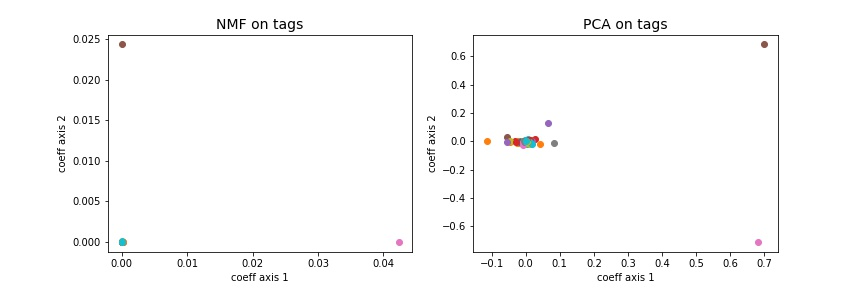
\includegraphics[width=\linewidth]{figures/analyse_exploratoire/product_PCA_coeffs.jpg}
\end{center}
\vfill
\end{overprint}
\end{frame}
%%%%%%%%%%%%%%%%%%%%%%%%%%%%%%%%%%%%%%%%%%%%%%%%%%%%%%%%%%%%%%%%%%%%%%
\begin{frame}{Produits - nombre de produit commandé}
\begin{center}
   \includegraphics[width=0.8\linewidth]{figures/analyse_exploratoire/products_nb_in_orders.jpg}
\end{center}
\end{frame}
%%%%%%%%%%%%%%%%%%%%%%%%%%%%%%%%%%%%%%%%%%%%%%%%%%%%%%%%%%%%%%%%%%%%%%
\begin{frame}{Produits - nombre d'apparition dans commandes}
\begin{center}
   \includegraphics[width=\linewidth]{figures/analyse_exploratoire/products_nb_apperance_log.jpg}
\end{center}
\end{frame}
%%%%%%%%%%%%%%%%%%%%%%%%%%%%%%%%%%%%%%%%%%%%%%%%%%%%%%%%%%%%%%%%%%%%%%
\begin{frame}{Produits - Réduction nb catégories}
\begin{itemize}
    \item Tentative clustering non supervisé
    \item Séparation par textmining et regroupement si premier mot commun : de $73$ à $49$ catégories
    \item Recherche information dans les variables numériques pour faire du target encoding : tentative de sélection des catégories avec une régression lasso sur les variables d'ACP\\
\end{itemize}

\vspace{0.5cm}
Pas de structure révélant les catégories mise en évidence. 
\end{frame}
%%%%%%%%%%%%%%%%%%%%%%%%%%%%%%%%%%%%%%%%%%%%%%%%%%%%%%%%%%%%%%%%%%%%%%
\begin{frame}{Produits - Extraction des variables}
\begin{center}
   \includegraphics[width=0.6\linewidth]{capture_ecran/product_dtypes.png}
\end{center}
\end{frame}
%%%%%%%%%%%%%%%%%%%%%%%%%%%%%%%%%%%%%%%%%%%%%%%%%%%%%%%%%%%%%%%%%%%%%%
%%%%%%%%%%%%%%%%%%%%%%%%%%%%%%%%%%%%%%%%%%%%%%%%%%%%%%%%%%%%%%%%%%%%%%
\subsection{Echelle Commande}
%%%%%%%%%%%%%%%%%%%%%%%%%%%%%%%%%%%%%%%%%%%%%%%%%%%%%%%%%%%%%%%%%%%%%%
%%%%%%%%%%%%%%%%%%%%%%%%%%%%%%%%%%%%%%%%%%%%%%%%%%%%%%%%%%%%%%%%%%%%%%
\begin{frame}{Exploration des tables - Commandes }
\begin{minipage}{0.4\linewidth}
        \begin{center}
           \includegraphics[width=\linewidth]{illustrations/graph_only_order.png}
        \end{center}
\end{minipage}
\begin{minipage}{0.58\linewidth}
\begin{itemize}
    \item Table \textit{orders} :
    \begin{itemize}
        \item[$\textendash$] Status de commande
        \item[$\textendash$] Dates d'achat et de livraison\\
    \end{itemize}
    \vspace{0.5cm}

    \item Table \textit{orders payments} : 
    \begin{itemize}
        \item[$\textendash$] Étalement des paiements
        \item[$\textendash$] Type de paiement
    \end{itemize}
\end{itemize}
\end{minipage}

\vspace{0.5cm}
\begin{minipage}{0.05\linewidth}
\hfill
\end{minipage}
\begin{minipage}{0.90\linewidth}
    \begin{itemize}
        \item Table \textit{order reviews}  (très creuse):
        \begin{itemize}
            \item[$\textendash$] Score de satisfaction
            \item[$\textendash$] Commentaire sur la satisfaction
        \end{itemize}
    \end{itemize}
\end{minipage}
\end{frame}
%%%%%%%%%%%%%%%%%%%%%%%%%%%%%%%%%%%%%%%%%%%%%%%%%%%%%%%%%%%%%%%%%%%%
\begin{frame}{Commandes - Status de commande}
\begin{center}
   \includegraphics[width=\linewidth]{figures/analyse_exploratoire/order_status.jpg}
\end{center}
\end{frame}
%%%%%%%%%%%%%%%%%%%%%%%%%%%%%%%%%%%%%%%%%%%%%%%%%%%%%%%%%%%%%%%%%%%%
\begin{frame}{Commandes - Dates}
\begin{center}
   \includegraphics[width=0.85\linewidth]{figures/analyse_exploratoire/order_time.jpg}
\end{center}
\end{frame}
%%%%%%%%%%%%%%%%%%%%%%%%%%%%%%%%%%%%%%%%%%%%%%%%%%%%%%%%%%%%%%%%%%%%
\begin{frame}{Commandes - Paiements}
\begin{center}
   \includegraphics[width=0.85\linewidth]{figures/analyse_exploratoire/order_payment.jpg}
\end{center}
\end{frame}
%%%%%%%%%%%%%%%%%%%%%%%%%%%%%%%%%%%%%%%%%%%%%%%%%%%%%%%%%%%%%%%%%%%%
\begin{frame}{Commandes - Extraction des variables}
\begin{center}
   \includegraphics[width=0.85\linewidth]{capture_ecran/orders_dtypes.png}
\end{center}
\end{frame}
%%%%%%%%%%%%%%%%%%%%%%%%%%%%%%%%%%%%%%%%%%%%%%%%%%%%%%%%%%%%%%%%%%%%
\begin{frame}{Commandes - Prétraitements statistiques}
    \begin{minipage}{0.52\linewidth}
        \begin{itemize}
            \item \textbf{Vectorisation des variables catégorielles }
            \item Passage à l'échelle logarithmique pour certaines variables
            \item Retrait des valeurs statistiquement aberrantes
            \item Inférence des variables manquantes
        \end{itemize}
    \end{minipage}
    \begin{minipage}{0.45\linewidth}
         "One Hot Encoder"
        \begin{itemize}
            \item date $\rightarrow$ 4 saisons
            \item heure $\rightarrow$ matin, après-midi, soir, nuit
            \item autres variables : type de paiement, ... 
        \end{itemize}
    \end{minipage}
\end{frame}
%%%%%%%%%%%%%%%%%%%%%%%%%%%%%%%%%%%%%%%%%%%%%%%%%%%%%%%%%%%%%%%%%%%%
\begin{frame}{Commandes - Prétraitements statistiques}
    \begin{minipage}{0.52\linewidth}
        \begin{itemize}
            \item Vectorisation des variables catégorielles 
            \item \textbf{Passage à l'échelle logarithmique pour certaines variables}
            \item Retrait des valeurs statistiquement aberrantes
            \item Inférence des variables manquantes
        \end{itemize}
    \end{minipage}
    \begin{minipage}{0.45\linewidth}
        Exemple avec 'price':
        \begin{center}
            \includegraphics[width=0.65\linewidth]{figures/analyse_exploratoire/orders_price_log_transfo.jpg}
        \end{center}
    \end{minipage}
\end{frame}
%%%%%%%%%%%%%%%%%%%%%%%%%%%%%%%%%%%%%%%%%%%%%%%%%%%%%%%%%%%%%%%%%%%%
\begin{frame}{Commandes - Prétraitements statistiques}
    \begin{minipage}{0.52\linewidth}
        \begin{itemize}
            \item Vectorisation des variables catégorielles 
            \item Passage à l'échelle logarithmique pour certaines variables
            \item \textbf{Retrait des valeurs statistiquement aberrantes}
            \item Inférence des variables manquantes
        \end{itemize}
    \end{minipage}
    \begin{minipage}{0.45\linewidth}
    Pour chaque variable :
        \begin{itemize}
            \item Si $val \leq Q_{0.05} - 1.5 \times IR$, 
                alors outlier inf\\ et 
                $val \leftarrow Q_{0.05} - 1.5 \times IR$
            \item Si $val \leq Q_{0.95} + 1.5 \times IR$, 
                alors outlier sup \\ et
                $val \leftarrow Q_{0.95} + 1.5 \times IR$
            \item Avec $IR = Q_{0.95} - Q_{0.05}$
        \end{itemize}
    \end{minipage}
\end{frame}
%%%%%%%%%%%%%%%%%%%%%%%%%%%%%%%%%%%%%%%%%%%%%%%%%%%%%%%%%%%%%%%%%%%%
\begin{frame}{Commandes - Prétraitements statistiques}
    \begin{minipage}{0.52\linewidth}
        \begin{itemize}
            \item Vectorisation des variables catégorielles 
            \item Passage à l'échelle logarithmique pour certaines variables
            \item Retrait des valeurs statistiquement aberrantes
            \item \textbf{Inférence des variables manquantes}
        \end{itemize}
    \end{minipage}
    \begin{minipage}{0.45\linewidth}
        Par KNN Impute : 
        \begin{center}
            \includegraphics[width=\linewidth]{figures/analyse_exploratoire/set_n_KNN_impute_orders.jpg}
        \end{center}
        $n\_neighbors = 6$
    \end{minipage}
\end{frame}
%%%%%%%%%%%%%%%%%%%%%%%%%%%%%%%%%%%%%%%%%%%%%%%%%%%%%%%%%%%%%%%%%%%%%%
%%%%%%%%%%%%%%%%%%%%%%%%%%%%%%%%%%%%%%%%%%%%%%%%%%%%%%%%%%%%%%%%%%%%%%
\subsection{Echelles Client}
%%%%%%%%%%%%%%%%%%%%%%%%%%%%%%%%%%%%%%%%%%%%%%%%%%%%%%%%%%%%%%%%%%%%%%
%%%%%%%%%%%%%%%%%%%%%%%%%%%%%%%%%%%%%%%%%%%%%%%%%%%%%%%%%%%%%%%%%%%%%%
\begin{frame}{Exploration des tables - Client }
\begin{center}
   \includegraphics[width=0.8\linewidth]{illustrations/graph_only_customers.png}
\end{center}
\begin{minipage}{0.33\linewidth}
    \begin{itemize}
        \item Table \textit{customers} :
    \end{itemize}
\end{minipage}
\begin{minipage}{0.65\linewidth}
    \begin{itemize}
        \item[$\textendash$] Signature unique des consommateurs
        \item[$\textendash$] Information géographique - Zip Code
    \end{itemize}
\end{minipage}
\begin{center}
   \includegraphics[width=0.8\linewidth]{figures/analyse_exploratoire/customer_location.jpg}
\end{center}
\end{frame}
%%%%%%%%%%%%%%%%%%%%%%%%%%%%%%%%%%%%%%%%%%%%%%%%%%%%%%%%%%%%%%%%%%%%
\begin{frame}{Client - Analyse RFM }
\begin{itemize}
    \item R = Recency :\\
    {\footnotesize \hspace{0.5cm} Quelle est la date du dernier achat pour ce client ?}
    \item M = Frequency :\\
    {\footnotesize \hspace{0.5cm} Quelle est la fréquence d'achat de ce client ?}
    \item F = Monetary Value :\\
    {\footnotesize \hspace{0.5cm} Combien ce client a-t-il dépensé sur le total de ses commandes ?}
\end{itemize}
\begin{center}
   \includegraphics[width=0.8\linewidth]{figures/analyse_exploratoire/boxplot_RFM.jpg}
\end{center}
\end{frame}
%%%%%%%%%%%%%%%%%%%%%%%%%%%%%%%%%%%%%%%%%%%%%%%%%%%%%%%%%%%%%%%%%%%%%%
%%%%%%%%%%%%%%%%%%%%%%%%%%%%%%%%%%%%%%%%%%%%%%%%%%%%%%%%%%%%%%%%%%%%%%
%%%%%%%%%%%%%%%%%%%%%%%%%%%%%%%%%%%%%%%%%%%%%%%%%%%%%%%%%%%%%%%%%%%%%%
\section{Modèles de ségmentation}
%%%%%%%%%%%%%%%%%%%%%%%%%%%%%%%%%%%%%%%%%%%%%%%%%%%%%%%%%%%%%%%%%%%%%%
%%%%%%%%%%%%%%%%%%%%%%%%%%%%%%%%%%%%%%%%%%%%%%%%%%%%%%%%%%%%%%%%%%%%%%
%%%%%%%%%%%%%%%%%%%%%%%%%%%%%%%%%%%%%%%%%%%%%%%%%%%%%%%%%%%%%%%%%%%%%%
\begin{frame}{Quel type de modèle ?}
    Modèles : Clustering non supervisé
    \begin{itemize}
        \item K-means
        \item DBSCAN
        \item Classification hierarchique
        \item Mélange de Gaussiennes\\
    \end{itemize}
    \vspace{0.5cm}
    Visualisation : Réduction de dimension non supervisée
    \begin{itemize}
        \item PCA
        \item NMF
        \item tSNE
    \end{itemize}
\end{frame}
%%%%%%%%%%%%%%%%%%%%%%%%%%%%%%%%%%%%%%%%%%%%%%%%%%%%%%%%%%%%%%%%%%%%%%
\begin{frame}{Sur quel type de données ?}
    Plusieurs échelles : 
    \begin{itemize}
        \item Client : Utiliser les axes RFM
        \begin{itemize}
            \item 3 dimensions
            \item 96096 clients
        \end{itemize}
        \item Commande : Utiliser le feature engineering de l'analyse exploratoire
        \begin{itemize}
            \item Grosse hypothèse : Perte de mémoire des clients
            \item 35 variables : Beaucoup plus d'information, grande dimension 
            \item 99441 commandes : jeu de données à pein plus gros
        \end{itemize}
    \end{itemize}
\end{frame}
% % %%%%%%%%%%%%%%%%%%%%%%%%%%%%%%%%%%%%%%%%%%%%%%%%%%%%%%%%%%%%%%%%%%%%%%
% % %%%%%%%%%%%%%%%%%%%%%%%%%%%%%%%%%%%%%%%%%%%%%%%%%%%%%%%%%%%%%%%%%%%%%%
\subsection{Recency Frequency Moneraty value}
% % %%%%%%%%%%%%%%%%%%%%%%%%%%%%%%%%%%%%%%%%%%%%%%%%%%%%%%%%%%%%%%%%%%%%%%
% % %%%%%%%%%%%%%%%%%%%%%%%%%%%%%%%%%%%%%%%%%%%%%%%%%%%%%%%%%%%%%%%%%%%%%%
\begin{frame}{RFM - Projection 3D et 2D}
    \begin{minipage}{0.48\linewidth}
        \begin{center}
           \includegraphics[width=\linewidth]{figures/models/RFM/RFM_3D_rotation1.jpg}
        \end{center}
    \end{minipage}
    \begin{minipage}{0.48\linewidth}
        \begin{center}
           \includegraphics[width=\linewidth]{figures/models/RFM/RFM_3D_rotation2.jpg}
        \end{center}
    \end{minipage}
    \begin{center}
       \includegraphics[width=\linewidth]{figures/models/RFM/RFM_2D_kmeans_8.jpg}
    \end{center}
\end{frame}
%%%%%%%%%%%%%%%%%%%%%%%%%%%%%%%%%%%%%%%%%%%%%%%%%%%%%%%%%%%%%%%%%%%%%%
\begin{frame}{RFM - Kmeans et clustering hiérarchique}
    
    \begin{minipage}{0.45\linewidth}
        kmeans :
        \begin{center}
           \includegraphics[width=\linewidth]{figures/models/RFM/RFM_kmeans_intertia.jpg}
           \includegraphics[width=\linewidth]{figures/models/RFM/rfm_yellowbricks_elbow.jpg}
           {\tiny avec Yellowbrick}
        \end{center}
    \end{minipage}
    \begin{minipage}{0.52\linewidth}
        Clustering hiérarchique\\
        \begin{center}
           \includegraphics[width=\linewidth]{figures/models/RFM/RFM_hclust_dendrogram2.jpg}
        \end{center}
    \end{minipage}

\end{frame}
%%%%%%%%%%%%%%%%%%%%%%%%%%%%%%%%%%%%%%%%%%%%%%%%%%%%%%%%%%%%%%%%%%%%%%
\begin{frame}{RFM - Kmeans et clustering hiérarchique}
    \begin{overprint}
        \onslide<1-> 
        \begin{center}
            Avec 5 clusters
           \includegraphics[width=\linewidth]{figures/models/RFM/RFM_2D_kmeans_5.jpg}
           \includegraphics[width=\linewidth]{figures/models/RFM/RFM_2D_hclust_5.jpg}
        \end{center}
            \onslide<2-> 
        \begin{center}            
            Avec 6 clusters
           \includegraphics[width=\linewidth]{figures/models/RFM/RFM_2D_kmeans_6.jpg}
           \includegraphics[width=\linewidth]{figures/models/RFM/RFM_2D_hclust_6.jpg}
        \end{center}
            \onslide<3-> 
        \begin{center}             
             Avec 7 clusters
           \includegraphics[width=\linewidth]{figures/models/RFM/RFM_2D_kmeans_7.jpg}
           \includegraphics[width=\linewidth]{figures/models/RFM/RFM_2D_hclust_7.jpg}
        \end{center}
            \onslide<4-> 
        \begin{center}             
            \textbf{Avec 8 clusters}
           \includegraphics[width=\linewidth]{figures/models/RFM/RFM_2D_kmeans_8.jpg}
           \includegraphics[width=\linewidth]{figures/models/RFM/RFM_2D_hclust_8.jpg}
        \end{center}
            \onslide<5-> 
        \begin{center}             
            Avec 9 clusters
           \includegraphics[width=\linewidth]{figures/models/RFM/RFM_2D_kmeans_9.jpg}
           \includegraphics[width=\linewidth]{figures/models/RFM/RFM_2D_hclust_9.jpg}
        \end{center}
        \onslide<6-> 
        \begin{center}             
            Avec 10 clusters
           \includegraphics[width=\linewidth]{figures/models/RFM/RFM_2D_kmeans_10.jpg}
           \includegraphics[width=\linewidth]{figures/models/RFM/RFM_2D_hclust_10.jpg}
        \end{center}
        \onslide<7-> 
        \begin{center}             
            Avec 11 clusters
           \includegraphics[width=\linewidth]{figures/models/RFM/RFM_2D_kmeans_11.jpg}
           \includegraphics[width=\linewidth]{figures/models/RFM/RFM_2D_hclust_11.jpg}
        \end{center}
    \end{overprint}
\end{frame}
%%%%%%%%%%%%%%%%%%%%%%%%%%%%%%%%%%%%%%%%%%%%%%%%%%%%%%%%%%%%%%%%%%%%%%
\begin{frame}{RFM - Autres modèles}
    \begin{overprint}
        \onslide<1->
            Gaussian mixture model : 
            \begin{center}             
               \includegraphics[width=0.8\linewidth]{figures/models/RFM/rfm_gmm.jpg}
            \end{center}
        \onslide<2->
            DBSCAN :
            \begin{center}             
               \includegraphics[width=0.9\linewidth]{figures/models/RFM/rfm_2D_DBSCAN1.jpg}
               \includegraphics[width=0.35\linewidth]{figures/models/RFM/rfm_2D_DBSCAN2.jpg}
            \end{center}
    \end{overprint}
\end{frame}
%%%%%%%%%%%%%%%%%%%%%%%%%%%%%%%%%%%%%%%%%%%%%%%%%%%%%%%%%%%%%%%%%%%%%%
%%%%%%%%%%%%%%%%%%%%%%%%%%%%%%%%%%%%%%%%%%%%%%%%%%%%%%%%%%%%%%%%%%%%%%
\subsection{Table des commandes}
%%%%%%%%%%%%%%%%%%%%%%%%%%%%%%%%%%%%%%%%%%%%%%%%%%%%%%%%%%%%%%%%%%%%%%
%%%%%%%%%%%%%%%%%%%%%%%%%%%%%%%%%%%%%%%%%%%%%%%%%%%%%%%%%%%%%%%%%%%%%%
\begin{frame}{Commandes - Réduction de dimension}
    \begin{center}             
       \includegraphics[width=0.9\linewidth]{figures/models/orders/orders_reduct_dim_pca.jpg}
    \end{center}
\end{frame}
%%%%%%%%%%%%%%%%%%%%%%%%%%%%%%%%%%%%%%%%%%%%%%%%%%%%%%%%%%%%%%%%%%%%%%
\begin{frame}{Commandes - K-Means}
    \begin{center}             
       \includegraphics[width=0.9\linewidth]{figures/models/orders/orders_kmeans_inertia.jpg}
    \end{center}
\end{frame}
%%%%%%%%%%%%%%%%%%%%%%%%%%%%%%%%%%%%%%%%%%%%%%%%%%%%%%%%%%%%%%%%%%%%%%
\begin{frame}{Commandes - Visualisation du clustering par PCA}
    \begin{overprint}
        \onslide<1-> 
            PCA - n\_clusters = 15
            \begin{center}             
                \includegraphics[width=\linewidth]{figures/models/orders/orders_PCA_kmeans_ncluster15.jpg}
            \end{center}
        \onslide<2->
            PCA - n\_clusters = 16
            \begin{center}             
                \includegraphics[width=\linewidth]{figures/models/orders/orders_PCA_kmeans_ncluster16.jpg}
            \end{center}
        \onslide<3->
            PCA - n\_clusters = 17
            \begin{center}             
                \includegraphics[width=\linewidth]{figures/models/orders/orders_PCA_kmeans_ncluster17.jpg}
            \end{center}
        \onslide<4->
            PCA - n\_clusters = 18
            \begin{center}             
                \includegraphics[width=\linewidth]{figures/models/orders/orders_PCA_kmeans_ncluster18.jpg}
            \end{center}
        \onslide<5->
            PCA - n\_clusters = 19
            \begin{center}             
                \includegraphics[width=\linewidth]{figures/models/orders/orders_PCA_kmeans_ncluster19.jpg}
            \end{center}
    \end{overprint}
\end{frame}
%%%%%%%%%%%%%%%%%%%%%%%%%%%%%%%%%%%%%%%%%%%%%%%%%%%%%%%%%%%%%%%%%%%%%%
\begin{frame}{Commandes - Visualisation du clustering par PCA}
    \begin{overprint}
        \onslide<1-> 
        tSNE -  n\_clusters = 15
            \begin{center}             
                \includegraphics[width=\linewidth]{figures/models/orders/orders_tSNE_kmeans_ncluster15.jpg}
            \end{center}
        \onslide<2-> 
        tSNE -  n\_clusters = 16
            \begin{center}             
                \includegraphics[width=\linewidth]{figures/models/orders/orders_tSNE_kmeans_ncluster16.jpg}
            \end{center}
        \onslide<3-> 
        tSNE -  n\_clusters = 17
            \begin{center}             
                \includegraphics[width=\linewidth]{figures/models/orders/orders_tSNE_kmeans_ncluster17.jpg}
            \end{center}
        \onslide<4-> 
        tSNE -  n\_clusters = 18
            \begin{center}             
                \includegraphics[width=\linewidth]{figures/models/orders/orders_tSNE_kmeans_ncluster18.jpg}
            \end{center}
        \onslide<5-> 
        tSNE -  n\_clusters = 19
            \begin{center}             
                \includegraphics[width=\linewidth]{figures/models/orders/orders_tSNE_kmeans_ncluster19.jpg}
            \end{center}
    \end{overprint}
\end{frame}

%%%%%%%%%%%%%%%%%%%%%%%%%%%%%%%%%%%%%%%%%%%%%%%%%%%%%%%%%%%%%%%%%%%%%%
\begin{frame}{Commandes - Pistes d'amélioration}
    \begin{itemize}
        \item Utiliser une NMF plutôt qu'une ACP comme réduction de dimension
        \item Utiliser d'autres méthodes de clustering : classification hierarchique, Gaussian Mixture Models
        \item Lancer le clustering directement dans l'espace réduit de tSNE
    \end{itemize}
\end{frame}

%%%%%%%%%%%%%%%%%%%%%%%%%%%%%%%%%%%%%%%%%%%%%%%%%%%%%%%%%%%%%%%%%%%%%%
%%%%%%%%%%%%%%%%%%%%%%%%%%%%%%%%%%%%%%%%%%%%%%%%%%%%%%%%%%%%%%%%%%%%%%
\subsection{Choix du modèle}
%%%%%%%%%%%%%%%%%%%%%%%%%%%%%%%%%%%%%%%%%%%%%%%%%%%%%%%%%%%%%%%%%%%%%%
%%%%%%%%%%%%%%%%%%%%%%%%%%%%%%%%%%%%%%%%%%%%%%%%%%%%%%%%%%%%%%%%%%%%%%
\begin{frame}{Meilleur modèle - Choix des données}
RFM - 8 clusters
    \begin{itemize}
        \item Consigne "facile d’utilisation pour l’équipe marketing"
            \begin{itemize}
                \item Séparation claire des clusters : représentation 3D
                \item Plus petit nombre de clusters : 8 VS 20
                \item Pas de pré-traitement
            \end{itemize}
    \end{itemize}
    \begin{center}
        \includegraphics[width=\linewidth]{figures/models/RFM/RFM_2D_hclust_8.jpg}
    \end{center}
\end{frame}
%%%%%%%%%%%%%%%%%%%%%%%%%%%%%%%%%%%%%%%%%%%%%%%%%%%%%%%%%%%%%%%%%%%%%%
\begin{frame}{Meilleur modèle - Choix du modèle}
    \begin{minipage}{0.51\linewidth}
        % \begin{itemize}
        % \item 
        Prop 1 : classification hiérarchique 
        \begin{itemize}
            \item Ajout online de nouveaux clients (coût mise en prod)
            \item Mise à jour bi-annuelle
            \item Stockage matrice distances
        \end{itemize}
        % \end{itemize}
    \end{minipage}
    \begin{minipage}{0.47\linewidth}
        % \begin{itemize}
        \item 
        % 
        Prop 2 : K-Means 
        \begin{itemize}
            \item Coût computation plus faible
            \item Mise à jour tous les 10 mois
            \item Performance $AMI = 58\%$
        \end{itemize}
        % \end{itemize}
    \end{minipage}
    
    \vspace{0.2cm}
    \begin{minipage}{0.45\linewidth}
        \begin{center}
            \includegraphics[width=0.92\linewidth]{figures/models/RFM/rfm_hist_frequency_diff.jpg}
        \end{center}
    \end{minipage}
    \begin{minipage}{0.06\linewidth}
    \hfill
    \end{minipage}
    \begin{minipage}{0.45\linewidth}
        \begin{center}
            \includegraphics[width=\linewidth]{figures/models/RFM/rfm_compare_cluster_training_size.jpg}
        \end{center}
    \end{minipage}
\end{frame}
%%%%%%%%%%%%%%%%%%%%%%%%%%%%%%%%%%%%%%%%%%%%%%%%%%%%%%%%%%%%%%%%%%%%%%
\begin{frame}{Meilleur modèle - Interprétation}
    \begin{center}
        \includegraphics[width=\linewidth]{figures/models/RFM/rfm_analyse_clusters.jpg}
    \end{center}
\end{frame}
%%%%%%%%%%%%%%%%%%%%%%%%%%%%%%%%%%%%%%%%%%%%%%%%%%%%%%%%%%%%%%%%%%%%%%
%%%%%%%%%%%%%%%%%%%%%%%%%%%%%%%%%%%%%%%%%%%%%%%%%%%%%%%%%%%%%%%%%%%%%%
%%%%%%%%%%%%%%%%%%%%%%%%%%%%%%%%%%%%%%%%%%%%%%%%%%%%%%%%%%%%%%%%%%%%%%
\section{Conclusion}
%%%%%%%%%%%%%%%%%%%%%%%%%%%%%%%%%%%%%%%%%%%%%%%%%%%%%%%%%%%%%%%%%%%%%%
%%%%%%%%%%%%%%%%%%%%%%%%%%%%%%%%%%%%%%%%%%%%%%%%%%%%%%%%%%%%%%%%%%%%%%
%%%%%%%%%%%%%%%%%%%%%%%%%%%%%%%%%%%%%%%%%%%%%%%%%%%%%%%%%%%%%%%%%%%%%%
\begin{frame}{Conclusion}
    Résumé
    \begin{itemize}
        \item Une analyse sur 3 échelles
        \item Deux façons de modéliser le problème
        \item Meilleur modèle = interprétabilité + facilité de calculs
    \end{itemize} 
    \vspace{0.2cm} 
    Améliorations et suite :
    \begin{itemize}
        \item Finir de faire un script avec le meilleur modèle en PEP8
        \item Utiliser la table "orders" pour caractériser les clusters de clients 
    \end{itemize}
    \vspace{0.5cm}
    \begin{center}
        {\Huge Merci pour votre écoute !}
    \end{center}
\end{frame}

\end{document}

